\documentclass[11pt,a4paper]{scrartcl}
\usepackage[czech]{babel}
\usepackage[utf8]{inputenc}
\usepackage{graphicx}
\usepackage{float}
\usepackage{amsmath}
\usepackage{subcaption}
\graphicspath{{./img/}}

\begin{document}
	\title{KIV/VSS}
	\subtitle{Simulace šíření lesího požáru buněčným automatem}
	\author{Zdeněk Valeš}
	\date{1.1. 2019}
	\maketitle
	\newpage
	
	\section{Zadání}
	Pomocí nástroje NetLogo naprogramujte simulaci lesního požáru. Základem pro semestrální práci bude existující příklad simulace v programu NetLogo, který rozšířím o další parametry (vítr, hořlavost terénu, typy terénu, jiný model šíření ohně, ...) tak, jak je popsáno v článku Simulation of forest fire fronts using cellular automata\cite{source_article}. Práce bude umět simulovat šíření ohnivé stěny i šíření ohně z předem vybraného bodu.Ideálně by práce měla umět načíst mapu ze souboru a na té provést simulaci.
	
	\section{Teorie}
	Práce implementuje model šíření lesního požáru celulárním automatem tak, jak byl navržen v \cite{source_article}. Původní simulace šíření požáru, která je dostupná v knihovnách NetLogu, byla založená na šíření ohně 'želvičkami'. Model navržený v článku předpokládá pouze buněčný automat a je vhodný po použití simulace homogenního i nehomogenního lesa (což je reálnější případ).
	
	\subsection{Model šíření ohně}
	Nejzákladnější model šíření ohně je založen na sčítání spálené plochy v osmi-okolí jedné buňky. Přírůstky od jednotlivých sousedů jsou násobeny koeficientem $\mu$, který v sobě zahrnuje parametry jako hořlavost, vítr, nebo výška terénu. V případě přilehlých sousedů je doba potřebná k úplnému spálení $t=\frac{L}{R}$ (naznačeno na obrázku \ref{fig:adj-model}), kde $L$ je rozměr plochy lesa (jedné 'buňky') a $R$ je hořlavost terénu.
	
	V článku je popsána první modifikace základního modelu (podle \cite{old_model_art}), která rozlišuje přírůstek spálené plochy od přilehlých a diagonálních sousedů. Tato modifikace plyne z předpokladu šíření ohně po úhlopříčce v případě diagonálních sousedů, viz obrázek \ref{fig:diag-model-old}.
	
	\begin{figure}[H]
		\centering
		\begin{subfigure}{0.3 \textwidth}
			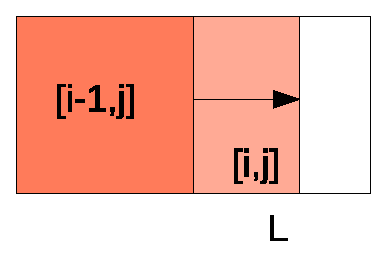
\includegraphics[width=\linewidth]{model-adj-spread}
			\caption{Model šíření ohnivé plochy z přilehlých sousedů}
			\label{fig:adj-model}
		\end{subfigure}
		\begin{subfigure}{0.3 \textwidth}
			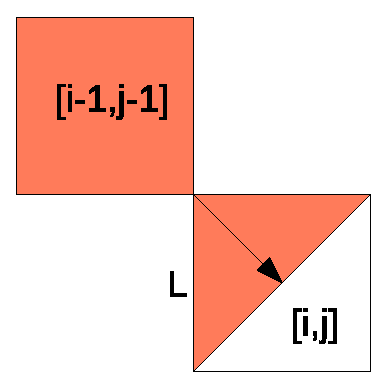
\includegraphics[width=\linewidth]{old-model-diag-spread}
			\caption{Starý šíření ohnivé plochy z diagonálních sousedů}
			\label{fig:diag-model-old}
		\end{subfigure}
		\begin{subfigure} {0.3 \textwidth}
			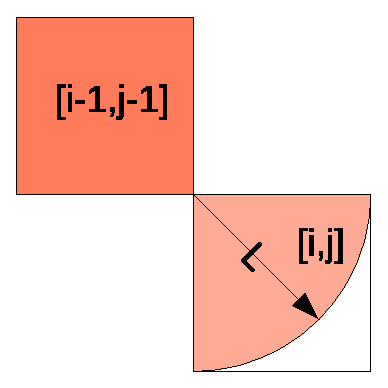
\includegraphics[width=\linewidth]{new-model-diag-spread}
			\caption{Nový model šíření ohnivé plochy z diagonálních sousedů}
			\label{fig:diag-model-new}
		\end{subfigure}
		\caption{Porovnání staršího a nového modelu šíření ohně z diagonálních sousedů}
	\end{figure}

	Tvůrci článku tento model dále posouvají a počítají spálenou oblast diagonálních sousedů jako část kruhu (viz obrázek \ref{fig:diag-model-new}). Podle tvůrců článku tento přístup více odpovídá realitě. U nového modelu tedy oheň z diagonálního souseda spálí za dobu $t$ plochu buňky rovnou $\frac{\pi L^2}{4L^2} \approx 0.785 \approx 78.5\%$.
	
	\paragraph{Parametry ovlivňující šíření ohně} Prvním parametrem je rychlost šíření $R [\frac{m}{s}]$, který popisuje hořlavost buňky. V případě nehomogenních lesů hraje v rovnici roli podíl $\frac{R_{i,j}}{R}$, kde $R$ je nejvyšší hořlavost v rámci simulovaného světa.
	
	Výška terénu, která je pro každou buňku popsána maticí $\Phi_{i,j}$ uvedenou v \ref{eq:height-matrix}. Oheň se po stoupajícím terénu šíří rychleji než po klesajícím \cite{source_article} a hodnoty v matici by tomu měly odpovídat: pokud terén klesá od severu k jihu, měly by hodnoty $h_{i-1,j-1}$,$h_{i,j-1}$, $h_{i+1,j-1}$ být vyšší než hodnoty zbytek hodnot v matici $\Phi_{i,j}$.
\begin{equation}
	\Phi_{i,j} =
	\begin{pmatrix}
	h_{i-1,j-1}       & h_{i,j-1} & h_{i+1,j-1} \\
	h_{i-1,j}       & 1 & h_{i+1,j} \\
	h_{i-1,j+1}       & h_{i,j+1} & h_{i+1,j+1} \\
	\end{pmatrix}
	\label{eq:height-matrix}
\end{equation}	
	
	Obdobně je řešen i vliv větru, který je popsán maticí $W_{i,j}$ uvedenou v \ref{eq:wind-matrix}. Matice funguje stejně, jako v případě matice s terénem. Pokud vítr fouká od severu k jihu, měly by hodnoty $w_{i-1,j-1}$,$w_{i,j-1}$, $w_{i+1,j-1}$ být větší než zbytek matice $W_{i,j}$.
	
	\begin{equation}
	W_{i,j} =
	\begin{pmatrix}
	w_{i-1,j-1}       & w_{i,j-1} & w_{i+1,j-1} \\
	w_{i-1,j}       & 1 & h_{i+1,j} \\
	w_{i-1,j+1}       & w_{i,j+1} & w_{i+1,j+1} \\
	\end{pmatrix}
	\label{eq:wind-matrix}
	\end{equation}	
	
	Po sestavení všech parametrů dohromady vznikne rovnice \ref{eq:fire-spread-eq}, která platí pro nehomogenní les. Parametry terénu a větru jsou zastoupeny koeficientem $\mu$, jehož přesný tvar je uveden v rovnici \ref{eq:mu}. Množiny $V_{adj}$ a $V_{diag}$ v sumách označují přilehlé, respektive diagonální okolí buňky.
	
	\begin{equation}
	a_{i,j}^{(t+1)} = \frac{R_{i,j}}{R}a_{i,j} + 
	\sum_{\alpha,\beta \in V_{adj}} \mu_{\alpha,\beta} \frac{R_{i + \alpha, j+\beta}}{R} a_{i + \alpha, j + \beta} ^{(t)} + 
	\sum_{\alpha,\beta \in V_{diag}} \mu_{\alpha,\beta} \frac{\pi R_{i + \alpha, j+\beta} ^2}{4R^2} a_{i + \alpha, j + \beta} ^{(t)}	
	\label{eq:fire-spread-eq}
	\end{equation}
	
	\begin{equation}
		\mu_{\alpha,\beta} = w_{i+\alpha, j+\beta} h_{i+\alpha, j+\beta}
		\label{eq:mu}
	\end{equation}
	
	Zbytek této kapitoly představuje přípravu na zkoušku.
	
	\subsection{Základy pravděpodobnosti}
	\begin{table}[H]
		\centering
		\begin{tabular}{|c|c|c|c|}
			\hline
			Název & Značení & Spojité & Diskrétní \\
			\hline
			\hline
			Střední hodnota & $E(X)$ & $\int{xf(x)}$ & $\sum s_ip_i$ \\
			\hline
			Rozptyl & $\sigma^2, D(X)$ & $\int{(x-E(X))^2p(x)}$& $\sum p_i(x_i - E(X))^2$ \\
			\hline
			Směrodatná odchylka & $\sigma, s_x$ & $\sqrt{D(X)}$ & \\
			\hline
			Variační koeficient & $v_x$ & $\frac{s_x}{\bar{x}}$ & \\
			\hline
		\end{tabular}
		\caption{Tabulka základních vzorečků}
	\end{table}

	\begin{table}[H]
		\centering
		\begin{tabular}{|c|c|c|c|c|}
			\hline
			Název & Hustota ppsti & Distribuční fce & Střední & Rozptyl \\
			& (PDF) & (CDF) & hodnota &  \\
			\hline
			\hline
			Rovnoměrné & $\frac{1}{b-a}$ & $\frac{x-a}{b-a}$ & $\frac{a+b}{2}$ & $\frac{1}{12}(b-a)^2$ \\
			\hline
			Normální & $\frac{1}{\sigma\sqrt{2\pi}}e^{-\frac{(x-\mu)^2}{2\sigma^2}}$ & $\frac{1}{\sqrt{2\pi}}e^{-\frac{x^2}{2}}$ & $\mu$ & $\sigma^2$ \\
			\hline
			
			Exponenciální & $\lambda e^{-\lambda x}$ & $1-e^{-\lambda x}$ & $\frac{1}{\lambda}$ & $\frac{1}{\lambda^2}$ \\
			\hline
			
			Poissonovo & $\frac{\lambda^x}{x!}e^{-\lambda}$ & exp. schody & $\lambda$ & $\lambda$ \\
			\hline
			Trojúhelníkové & $0$ pro $x < a$ & $0$ pro $x \le a$  & $\frac{a +b +c}{3}$& $\frac{a^2+b^2+c^2-ab-ac-bc}{18}$ \\
			
			(a-c-b) & $\frac{2(x-a)}{(b-a)(c-a)}$ pro $x < c$ & $\frac{(x-a)^2}{(b-a)(c-a)}$ pro $x \le c$ & & \\
			
			 & $\frac{2}{(b-a)}$ pro $x = c$ & & & \\
			 & $\frac{2(b-x)}{(b-a)(b-c)}$ pro $x \le b$ &  $1- \frac{(b-x)^2}{(b-a)(b-c)}$ pro $c < b$ & & \\
			 & $0$ pro $x > b$ & $1$ pro $x \ge b$  & & \\
			\hline
		\end{tabular}
		\caption{Tabulka se vzorečky pro základní rozdělení}
	\end{table}
	
	\subsection{Generování náhodných čísel}
	\begin{itemize}
		\item Kvazirozměrné rozložení, generátor uniformního rozložení (celé číslo na n bitech)
		
		\item Metoda prostředních čtverců
		
		\item Lineární rovnice + modulo aritmetika ($y_{i+1}= (ay_i +c) \; mod \; m$)
	\end{itemize}

	\subsubsection{Generování dalších rozdělení}
	
	\paragraph{Transformační metoda}
	Uniformní rozdělení transformujeme podle inverzní distribuční fce $F^{-1}(u)$. Vhodné pokud je $F^{-1}(u)$ snadno zjistitelná.


	\paragraph{Vylučovací metoda}
	Musí být známa hustota ppsti $f(x)$. Dvěma uniformními generátory dostanu čísla v prostoru: 
	
	\begin{itemize}
		\item $G_1$ s uniformním rozdělením na <a,b>
		
		\item $G_2$ s uniformním rozdělením na <0,M>
		
		\item $G_1 => y_1 => x_i = (b-a)y_1 + a$
		
		\item $G_2 => y_2 => z_i = My_2$
		
		\item Pokud $z_i < f(x_i)$ pak $x_i$ je náhodné číslo s rozdělením f(x); jinak opakuj
	\end{itemize}

	\paragraph{Obecné diskrétní rozdělení}
	Pokud znám schodovou distribuční fci, generuji 1 číslo s uniformním rozdělením podle tabulky (CDF) určím výslednou hodnotu.

	\subsubsection{Generování normálního rozdělení}
	Součet $n$ náhodných čísel s rovnoměrným rozdělením se asymptoticky blíží k normálnímu rozdělení. $s_n = \sum_{1}^{n}y_i$, hodí se volit $n = 12$ protože $E\{s_n\} = nE\{y_i\} = \frac{n}{2} = 6$ a $D\{s_n\} = nD\{y_i\} = \frac{n}{12} = 1$, je tedy snadné generovat gaussovo rozdělení se $\mu=6$ a $\sigma=1$. Pro zadané $\mu$ a $\sigma$: $\sigma\cdot(\sum_{i=1}^{12} y_i -6) +a$
	
	\paragraph{Box-Müllerova transformace}
	Stačí dvě hodnoty $x_1$,$x_2$ s normovaným rovnoměrným rozdělením: 
	\begin{itemize}
		\item $z_1 = \sqrt{-2ln(-x_1)}cos(2\pi x_2)$
		\item $z_2 = \sqrt{-2ln(-x_1)}sin(2\pi x_2)$
	\end{itemize}
    
    Lze ještě aplikovat parametry normálního rozdělení: $z_1 \sigma \mu $.
	
	\subsubsection{Testování generátoru} 
	Ověřit, zda má generátor zadané vlastnosti (střední hodnotu, rozptyl, délka periody ...).
	
	\paragraph{$\chi^2$ test} Testuji, že nějaká hypotéza neplatí (nebo, že ji nelze zamínout). 
	
	\begin{itemize}
\item 	Hodnoty z $\{y_i\}_1^n$ rozdělím do $k$ intervalů. V každém intervalu spočtu četnost $\theta_i$, ppst $p_i$, že hodnota $y_i$ spadne do intervalu. 

\item  $\chi^2=\sum_{i=1}^{k} \frac{(\theta_i - np_i)^2}{np_i}$
\item Porovnání s tabulkovou hodnotou. $\chi^2 \le \chi_{tab}^2$ pak hypotézu nelze zamítnout. Jinak hypotézu zamítnu na hladině ppsi $\alpha$.
	\end{itemize}
	
	\subsection{Markovské náhodné procesy}
	Poissonovo (počet jevů v určitém čas. intervalu) vs. Exponenciální rozdělení (délka intervalu mezi dvěma událostmi).
	
	\begin{itemize}
		\item Stř. doba setrvání ve stavu $i$: $T_i=\frac{1}{\lambda_i}$
		\item Stř. frekvence přechodů po hraně z $i$ do $j$: $f_{i,j}=p_i\cdot\lambda_{i,j}$ (pouze bez abs stavů)
		\item Stř. doba cyklu průchodů stavem $i$: $T_{ci} = \frac{1}{f_i}$ (pouze bez abs stavů)
	\end{itemize}
	
	\subsection{Systémy hromadné obsluhy}
	Vstupní proud: $a$,$\lambda$. Doby obsluh: $s$,$\mu$. Fronta: $w$. Celý systém: $q$. Doba: $T$,$t$ (velká písmena = stř hodnoty, malá konkrétní). Počet požadavků: $L$. Zátěž systému: $
	\rho = 
	\frac{T_{obsluha}}{T_{mezi \; prichody}} = \frac{T_s}{T_a}$. Pokud $\rho < 1$, pak se jedná o stacionární režim (systém není přetížený).
	
	\paragraph{Charakteristiky vstupního proudu}
	Veličina $\tau$. Exponenciální proud lze popsat jedním parametrem $\lambda$, proto $E\{\tau\} = T_a = \frac{1}{\lambda}$ (viz vzorečky ppsti). Koeficient variace určuje, jak moc je proud náhodný, typicky v intervalu $<0;1>$, kde $0$ jsou pravidelné příchody. Výstupní porud má stejnou periodu a frekvenci jako vstupní (pro stac. režim). Jinak $m\cdot\mu$ a rozdělení se blíží $F_s(t)$.
	
	\paragraph{Fronta požadavků}
	Aktuální počet požadavků ve frontě: $w$. Střední počet požadavků ve frontě $L_w$. Doba čekání jednoho požadavku $t_w$. Stř. doba čekání požadavku ve frontě $T_w$. 

	\paragraph{Charakteristiky SHO} $T_s = \frac{1}{\mu}$. Mezi středními hodnotami platí následující vztahy.
	Stř. počet prvků v systému: $L_q = L_w + L_s = L_w + m\frac{\lambda}{\mu}$.
	Stř. doba průchodu systémem: $T_q = T_w + T_s = T_w + \frac{1}{\mu}$.
	
	Littleovy vzorce:
	\begin{itemize}
		\item $L_q = \lambda \cdot T_q$
		\item $L_w = \lambda \cdot T_w$
		\item $T_w = L_w \cdot T_a$
	\end{itemize}
	
	
	\subsubsection{Kendallova klasifikace}
	Znám charakteristiku vstupního proudu $F_a(t)$ a kanálu obsluhy $F_s(t)$, chci určit vlastnosti systému. Systém fron popsán pěticí X/Y/m(/I/disc)
	\begin{itemize}
		\item \textbf{X}: prvd. rozdělení vstupního produ
			\subitem GI = obecné náhodné rozdělení, stat nezáv.; G = obecné náhodné rozdělení; M = exponenciální rozdělení; D = determ. intervaly
		\item \textbf{Y}: prvd. rozdělení dob obsluh
		\item \textbf{m}: počet kanálů obsluhy
		\item \textbf{I}: max. délka fornty (obvykle $\infty$).
		\item \textbf{disc.}: frontová disciplína (obvykle FIFO).
	\end{itemize}
	 
	\paragraph{M/M/1}
	Nejjednodušší případ, charakterizováno parametry $\lambda$,$\mu$. $\rho = \frac{\lambda}{\mu}$, pro stac. režim $\lambda < \mu$. Pokud stacionární, lze modelovat jako mark. proces: $p_k=\rho^kp_0=\rho^k(1-\rho)$. $E\{k\} = L_q = \sum_{k=0}^{\infty} kp_k = (1-\rho)\frac{\rho}{(1-\rho)^2}$.
	
	\paragraph{M/M/m}
	$m$ obslužných kanálů pro 1 frontu.
	Koeficient vytížení: $\rho=\frac{1}{m}\frac{\lambda}{\mu}=\frac{1}{m}\frac{T_s}{T_a}=\frac{\lambda T_s}{m}$. Pro $m\in\{1,2\}$ přesný, jink pouze přibližný odhad: $L_q=\frac{m\rho}{1-\rho^m}$; $T_q=\frac{T_s}{1-\rho^m}$.
	
	Pokud konečná fronta, některé požadavky zahozeny, proto nelze použít vzorce pro nekonečnou délku fronty a proto platí, že $\lambda_{realne} < \lambda_{teoreticke}$. Vzorce pro konkrét í případ lze odvodit z mark. modelu.
	
	\paragraph{M/G/1}
	Nemarkovský model. Potřebuji $\lambda$ pro vstupní proud a $F_s(t)$, nebo $f_s(t)$ pro popis doby obsluhy. $\rho = \lambda T_s$ kde $T_s$ je stř. doba rozdělení $F_s(t)$. Na zbytek potřebuji koef. variace ($C_s^2$). $C_s = \frac{\sigma(\tau)}{T_s}$.
	
	\begin{itemize}
		\item $L_w = L_{w(M/M/1)}\frac{1+C_s^2}{2}=\frac{\rho^2}{1-\rho}\frac{1+C_s^2}{2}$
		
		\item $L_q = L_w + L_s (=L_w + \frac{\lambda}{\mu} = L_w + \rho)$
		
		\item $T_q = \frac{L_q}{\lambda}$
		
		\item $T_w = \frac{L_w}{\lambda}$;$T_w = T_q - T_s$
	\end{itemize}
	Markovské modely se používají jako odhad nejhoršího průběhu.
	
	\paragraph{GI/G/1} Stat. nezávislost dob příchodů ve vstupu. Potřebujeme znát $F_a(t)$, nebo $f_a(t)$. Zatížení $\rho = \frac{T_s}{T_a}$. Příbližně $L_w=\frac{\rho^2}{1-\rho}\frac{C_a^2+C_s^2}{2}$. Pro D/D/1 je $L_w=0$ pokud je $T_a > T_s$. Pro M/M/1 je $\frac{C_a^2+C_s^2}{2} = 0$.
	
	
	\subsubsection{Složené sítě}
	Jsou-li všechny vstupní toky poissonovské a obsluhy exponenciální, jsou i výstupní toky exponenciální. $\rightarrow$ dílčí SHO lze řešit jako M/M/m. Littleův zákon: $\L_q = \Lambda_0\cdot T_q$ (v podstatě: co do sítě vstoupí z ní musí i vystoupit). $\Lambda_0$ je souhrný vstupní tok do systému, $\Lambda_i$ vnitřní frekvence toku v uzlu. Pro uzly ve stacionárním systému platí obdoba Krichhoffových zákonů (z nich lze pak zjistit $\Lambda_i$). Zatížení uzlu: $\rho_i = \frac{1}{m_i}\Lambda_i T_{si}$. Pokud každé $\rho_i < 1$, pak je systém stacionární.
	
	Uzavřené sítě front lze řešit převedením na markovský model. V případě modelů interaktivního systému (n terminálů, 1 fronta, 1 server) se přechody do prava postupně zmenšují ($n\lambda$, $(n-1)\lambda$, ..., $\lambda$). Propustnost pak je $x=\frac{1}{T_s}(1-p_0)$ (ve stavu $p_0$ není co obsluhovat). $T_q=(n\frac{T_s}{1-p_0}) - T_t$ ($T_t = \frac{1}{\lambda}$ je doba 'přemýšlení' terminálu). 
	
	\paragraph{Nepoissonovské sítě front} Toky obecně charakterizovány $\lambda$ a variačním koef. $C_\tau$. Pro stacionární platí $\lambda_{in} = \lambda_{out}$. Platí $C_{out}^2=1+\rho^2(C_s^2-1)+(1-\rho^2)(C_\tau^2-1)$. $\rho$ určuje vliv rozdělení dob vstupů a dob obsluh. Tok s $\lambda$,$C_\tau$ lze dělit na $n$ toků: $\lambda_i = \lambda p_i$, $C_i^2 = 1 + p_i(C_\tau^2-1)$. Slučovat toky lze podle: $\lambda = \sum_{i=1}^{n}\lambda_i$,$C^2 = 1+\sum_{i=1}^n(\frac{\lambda_i}{\lambda})^2(C_i^2 - 1)$. Pro jednotlivé elementární SHO lze použít vztahy pro GI/G/n.
	
	\subsection{Základy teorie spolehlivosti} Systematické (bugy) vs. náhodné poruchy. Opravitelné vs. neopravitelné systémy. Zálohy: cold (vypnutá, aktivuje se po výpadku), teplá (zapnutá, neaktivní až do výpadku), horká (paralelně s hlavním výpočtem). MTTF = střední doba do poruchy (v modelech často $\lambda = \frac{1}{MTTF}$). MTBF = střední doba mezi poruchami. MTTR střední doba do opravy (v modelech často $\lambda = \frac{1}{MTTR}$).
	
	\paragraph{Ukazatele spolehlivosti} $Q(t)$ je distribuční fce ppsti poruchy. $R(t) = 1 Q(t)$ je distribuční fce ppsti bezporuch. provozu. Hustota ppsti: $f(t)$. Intenzita poruch: $\lambda(t) = \frac{f(t)}{R(t)}$. Výpočty vychází z empiricky zjištěné vanové křivky (čeká se na ustálení systému kdy je $\lambda$ cca konstantní), pak platí:
	\begin{itemize}
		\item $R(t) = e^{-\lambda t}$
		\item $Q(t) = 1 - e^{-\lambda t}$ (distrib. fce exp. rozdělení)
		\item $f(t) = \lambda e^{-\lambda t}$ (hustota ppsti exp. rozdělení)
	\end{itemize}

   Neobnovované objekty: $T_s = \frac{1}{\lambda}$. Obnovované objekty: $T_s = \frac{t_p}{n} = \frac{1}{n} \sum_{i=1}^{n} \tau_{pi}$ kde $\tau_{pi}$ jsou dby jednotlivých poruch. Obdobně střední doba cyklu (MTBF) je $T_c = \frac{1}{n} \sum_{i=1}^{n} (\tau_{pi} + \tau_{oi})$. Ppst, že objekt bude fungovat v libovolné době (koeficient pohotovosti): $K_p = \frac{t_p}{t_p + t_o}$. MTTR lze zavést jako $T_o = \frac{t_o}{n}$ (pro exp. $\frac{1}{\mu}$). $K_p = \frac{T_s}{T_s+T_q}=\frac{\mu}{\lambda + \mu}$. Součinitel prostoje: $K_n(t) = 1-K_p(t)$.
	
	\paragraph{Systémy s nezávislými prvky} Paralelní vs. sériové zapojení prvků. Pro sériové platí: $R(t) = \Pi_{i=1}^n R_i(t)$, $T_s = \frac{1}{\sum_{i=1}^{n}\lambda_i}$. Pro paralelní zapojení platí: $Q(t) = \Pi_{i=1}^n Q_i(t)$. V případě kombinovaných zapojení postupně redukuji. Pro exp. doby poruch platí: $T_s=\int_{0}^{\inf} R(t)dt = \frac{1}{\lambda_1+...} + \frac{1}{\lambda_1+...}$ (integruju $e^{-(\lambda_1+..)t}$ podle $t$). Mohu použít stavový graf, je $n$ prvků, musí fungovat alespoň $k$. Pro výsledné $R$ sečtu všechny stavy ($R_1 R_2 R_3$ pro stav $111$, $R_1Q_2R_3$ pro stav $101$, ...).
	
	\paragraph{Markovský model pro neob. systém} Podle problému vytvořím graf. Najdu všechny cesty z $1.$ do $n$ (absorpčního stavu), pro každou cestu určím $T_{ci}$ a $p_{ci}$. $T_s = \sum T_{ci} p_{ci}$. $T_ci$ určím jako součet $\frac{1}{\sum \lambda_{odchozi}}$ pro každou hranu v cestě. $p_ci$ určím jako součin $\frac{\lambda_{hrana}}{\sum \lambda_{odchozi}}$ pro každou hranu v cestě.
	
	\paragraph{Markovský model pro ob. systém} Klasika. $K_p = \sum_{ok \; stavy} p_i$, $T_s = \frac{\sum_{ok \; stavy}}{ppst \; prechodu \; do \; neok \; stavu}$.
	
	
	\subsection{Diskrétní stochatické modely} Stochastická = založena na náhodných číslech. Diskrétní = stav jen v diskrétních okamžicích. Událostní = čas založený na událostech (ne na pravidelném korku). Stoch. simulace = výsledky se blíží realitě s větším počtem pokusů (Buffonova jehla).
	
	\paragraph{Metoda pseudoparalelních procesů} Založeno na objektové dekompozici simulačního modelu. Aktivní objekty = pracují podle vlastního programu; Pasivní objekty = poskytují služby ostatním. Základní objekty pro simulaci:  prvek seznamu (\textbf{LINK}) = objekt, který lze řadit do seznamů. Hlava seznamu (\textbf{HEAD}) = objekt reprezentující seznam. Proces (\textbf{PROCESS}) = aktivní prvek, může vykonávat činnost (generátory, kanály obsluhy).
	
	\textbf{LINK}:
	\begin{itemize}
		\item into(seznam) vloží objekt do zadaného seznamu
		\item follow(prvek) zařadí objekt za daný prvek do seznamu
		\item precede(prvek) zařadí objekt před daný prvek
		\item out() vyjme prvek ze seznamu
	\end{itemize}

   \textbf{HEAD}:
   \begin{itemize}
		\item empty() je prázdný
		\item cardinal() jak je velký
		\item first() první prvek
		\item last()
		\item clear()
   \end{itemize}

	Prvky propojuji tak, že nový liunk přidám do fronty následujícího uzlu (přímá reference vs. všchny prvky v hash + identifikátor). Jednotný interface pro uzly akceptující požadavky (accept(link)), zpracování závisí na daném objektu. Kanál obsluhy zpožďuje cestu požadavku v síti (metoda hold(time)).
	
	\paragraph{Měření charakteristik sítě} Doba průchodu systémem $T_q$: pro každý prvek času vstupu do systému a čas výstupu ze systému $\rightarrow$ mohu počítat E(x), D(x) a histogram. 
	
	Statistika toku v místě: počítám rozdíl času v accept(). Mohu zjišťovat délky front $L_q$,$L_w$ (vzorkování). Zatížení serveru: $\rho = \frac{doba \; obsluh}{celkova \; doba}$.
	
	\paragraph{Mechanismus bariéry} Proces: střídání hold() a barrier.arrived(this). Bariéra: Postupně čeká až přijdou všechny procesy, pak všechny aktivuje.
	
	\paragraph{Bariéra + KS (randez-vous)} Proces: střídání hold() a barrier.arrived(this). Bariéra: Postupně čeká až přijdou všechny procesy, pak proběhne KS (hold()), pak se uvolní všechna vlákna.
	
	\paragraph{Monitor} KS se spouští pro každé vlákno ale smí v ní být jen jedno. Proces: hold($\lambda$); section.enter(); hold($\mu$); section.exit(). Monitor: nové procesy uspí, pokud je KS obsazená, při odchodu procesu probere první čekající.
	
	\paragraph{Producent, konzument} Producent: Dává (produkce = hold()) linky do bufferu, dokud může, pak se uspí. Pokud je něco v bufferu, vzbudí konzumenta. Konzument: pokud je buffer prázdný, uspí se. Jinak konzumuje. Pokud je buffer prázdný a producent spí, vzbudí jej. Konzumace = hold().
	
	\subsection{Benchmarky} Benchmark musí být opakovatelný a měřitelný. Dělení od nejsložitějších ale nejpřesnějších k nejsnáze naimplementovatelným: program, kvli kterému testujeme $\rightarrow$ reálné programy $\rightarrow$ jádra $\rightarrow$ syntetické benchmarky $\rightarrow$ specifické algoritmy.
	
	\paragraph{Hodnocené vlastnosti} Rychlost (odezva, MIPS), Spolehlivost, Dostupnost, Cena. Typické metriky: čas (něčeho), kapacita (celého/části systému), výkon (efektivita), spolehlivost (MTBF), dostupnost (MTTF, MTTR). Reálná vs. syntetická zátěž. Parametry = předem dané, faktor = parametry zátěže měnící se v čase.
	
	\paragraph{Návrh testu} S minimálním úsilím získat co nejvíc informací. Přesný popis zátěže a posloupnosti kroků. Přesná volba cílů (z toho vychází volba testů a interpretace výsledků). Systém = souhrn použitého SW,HW. Uživatel = netita využívající systém. Metrika = kritérium zvolené pro hodnocení, Zátěž = požadavky zasílané uživateli. Měření na reálném systému vs. analytický model vs. simulace. 
	
	\paragraph{Příklady benchmarků} Erastothenovo síto: hledání prvočísel, výkon zvisí na rychlosti paměti, implementaci polí, velikosti cache. Ackermanova funkce: test schopnosti překladače optimalizovat rekurzi. Whetstone (1972 - staré): sada instrukcí podle statistiky (50\% jump, 30\% aritmetika, ...) pro vědecké programy, měří počet float instrukcí za sekundu. Závisí na kvalitě překladače. Dhrystone (1984): realističtější než wheatstone (=použita jiná statistika pro instrukce), měří cykly/s nebo MIPS. CoreMark (2009): zpracování seznamů, matice, konečný automat, CRC, vlastní skóre.Linpack: řešení float soustavy lin. rovnic gauss. metodou, TFLOPS, porovnání superpočítačů. Debit/Credit: test databází, v každé transakci zápis do 4 tabulek, cena/1 transakci (TPC-C V5 modernější). SPEC Suite: sada různých reálný programů, testují různé komponenty/vlastnosti PC (pro Javu SPEC JVM2008). PCMark(domácí PC), 3DMark (grafické karty)
	
	
	\paragraph{Základní chyby} Korelace není kauzalita. Aritmetický průměr vs. harmonický průměr (lepší pro převrácené hodnoty). Špatná tvorba grafu (měřítko, počátek os, popis os, špatný typ grafu). Porovnávání výsledků různých benchamrků. Povaha benchmarku neodpovídá povaze reálného použití stroje/SW. Nesystematický přístup (např. při volbě parametrů). Nevhodně zvolená zátěž systému. Benchmark je známý a výrobci pro něj optimalizují.
	
	\section{Svět interpretovaný v NetLogu}
	Svět simulovaný v NetLogu se rozkládá na ploše 256x256 pixelů. Jeden pixel odpovídá čtvercové ploše 10x10 metrů v reálném světě. Model v článku počítá s časovým krokem určeným podle hořlavosti terénu, v mé implementaci je časový krok konstantní (1 minuta) a hořlavost je zadávána v rozmezí $<0;1> \frac{m}{min}$. Vzhledem k tomu, že jedna buňka mého modelu má rozměr 10m, je takto zadaná hořlavost vydělena 10. Pokud tedy buňka s hořlavostí 1 bude mít jednoho přilehlého, úplně vyhořelého souseda, je doba potřebná k jejímu vyhoření 10 minut (tiků). 
	
	
	Popis světa (1 tik = 1 minuta, 1 buňka = 10x10 m, šíření ohně, ...)
	
	Obrázek aplikace matice větru a terénu
	
	\subsection{Popis programu}
	\begin{figure}
		\centering
		\caption{Vývojový diagram procedury go}
		\label{fig:go-procedure}
	\end{figure}
	
	
	\section{Použití}
	Možnost nahrávat mapy z obrázků. Možnost nastavení hořlavosti druhů terénu, možnost nastavení matice výšky terénu.
	
	\section{Testování}
	Testy v článku, obrázky z mého programu, srovnání
	
	\section{Závěr}
	
	\begin{thebibliography}{9}
		
		\bibitem{source_article}
		ENCIAS, Hernández a WHITE, Hoya a del RAY, Martín a SANCHÉZ, Rodríguez . Simulation of forest fire fronts using cellular automata. \textit{Advances in Engineering Software: Advances in Numerical Methods for Environmental Engineering}. 2007, 2007(6), 372-378. ISSN 0965-9978. Dostupné také z: https://www.sciencedirect.com/science/article/pii/S0965997806001293
		
		\bibitem{old_model_art}
		KARAFYLLIDIS, Ioannis a THANAILAKIS, Adonios. A model for predicting forest fire spreading using cellular automata. \textit{Ecol Model} 1997, 99, 87–97.
	\end{thebibliography}
	
\end{document}
